
\clearpage
\section{Window Size Parameter}
\label{secX:windows}

In this section we analyze \textbf{how much does / the extent to which} the window size parameter affects the performance of the algorithms. We only consider the four datasets that consist of multiple files, i.e. \datasetirkis, \datasetsst, \datasetadcp \ and \datasetsolar. For every data type in each dataset file we compare the compression ratios obtained when using the optimal global window size and the optimal local window size (for that data type in that file). 

For example, in Figure~\ref{fig:window-compare-1202} we display the compression ratio and relative difference plots obtained for the ``VWC" data type of the ``vwc\_1202.dat.csv" file. We can see, for instance, that in the CoderAPCA case both window size parameters match for every threshold parameter $e$, except 3 and 10. When $e=3$ the optimal global window size is larger, and when $e=10$ the optimal local window size is larger. In those cases the relative differences are 1.52 and 1.76, respectively. Notice that in every plot the relative difference is non-negative, which was expected, since the compression rate obtained when using the optimal global window will never be smaller than the compression rate obtained when using the optimal local window.

Table~\ref{tabla:windows-comparison} summarizes the results obtained for each combination of algorithms, threshold parameters, data types and files, sorted by algorithm. In 88.7\% of the cases both window sizes match, and so the relative difference is 0. In the remaining cases, most of the times the relative difference is smaller than 1, and there are only six cases in which the relative difference is larger than 5.

\vspace{+10pt}




\begin{table}[h]

\begin{center}

    \begin{tabular}{| C{2.5cm} || C{2.2cm} | C{1.5cm} | C{1.5cm} | C{1.5cm} | C{1.5cm} |}

    \hline

    \multicolumn{1}{|>{\centering\arraybackslash}m{2.5cm}||}{}

    & \multicolumn{5}{>{\centering\arraybackslash}m{9cm}|}{RD (\%) Range}\\

    \hline

      \multicolumn{1}{|>{\centering\arraybackslash}m{2.5cm}||}{\textbf{Algorithm}}

    & \multicolumn{1}{>{\centering\arraybackslash}m{2.2cm}|}{\textbf{0}}

    & \multicolumn{1}{>{\centering\arraybackslash}m{1.5cm}|}{\textbf{(0,1]}}

    & \multicolumn{1}{>{\centering\arraybackslash}m{1.5cm}|}{\textbf{(1,2]}}

    & \multicolumn{1}{>{\centering\arraybackslash}m{1.5cm}|}{\textbf{(2,5]}}

    & \multicolumn{1}{>{\centering\arraybackslash}m{1.5cm}|}{\textbf{(5,11]}}\\

    \hline\hline

    PCA & 186 (93\%) & 3 (1.5\%) & 4 (2\%) & 2 (1\%) & 5 (2.5\%) \\\hline
    APCA & 174 (87\%) & 13 (6.5\%) & 7 (3.5\%) & 6 (3\%) & 0 \\\hline
    CA & 172 (86\%) & 16 (8\%) & 6 (3\%) & 6 (3\%) & 0 \\\hline
    FR & 171 (85.5\%) & 14 (7\%) & 8 (4\%) & 7 (3.5\%) & 0 \\\hline
    PWLH & 184 (92\%) & 13 (6.5\%) & 3 (1.5\%) & 0 & 0 \\\hline
    PWLHInt & 180 (90\%) & 8 (4\%) & 9 (4.5\%) & 3 (1.5\%) & 0 \\\hline
    GAMPS & 167 (83.5\%) & 15 (7.5\%) & 11 (5.5\%) & 3 (1.5\%) & 4 (2\%) \\\hline
    SF & 199 (99.5\%) & 1 (0.5\%) & 0 & 0 & 0 \\\hline\hline
    Total & 1,433 (89.5\%) & 83 (5.2\%) & 48 (3\%) & 27 (1.7\%) & 9 (0.6\%) \\\hline
    \toprule[0.1mm]

    \end{tabular}

    \caption{RD between the \ows and \lows variants of each CAI.\\The results are aggregated by algorithm and the range to which the RD belongs.}

    \label{tabla:windows-comparison}

\end{center}

\end{table}


\vspace{-5pt}

In Figure~\ref{fig:window-compare-1203} we display the plots obtained for the ``VWC" data type of the ``vwc\_1203.dat.csv" file. For CoderPCA and $e=15$ the relative difference is 10.68, which is the largest value obtained for all of the combinations. The next four largest relative differences (9.79, 9.22, 7.20, and 5.51) are also obtained with the CoderPCA algorithm. These results support the idea that the performance of the CoderPCA algorithm is more sensible to the window size parameter than the rest of the algorithms.

\clearpage

\begin{figure}
\hspace{-70pt}
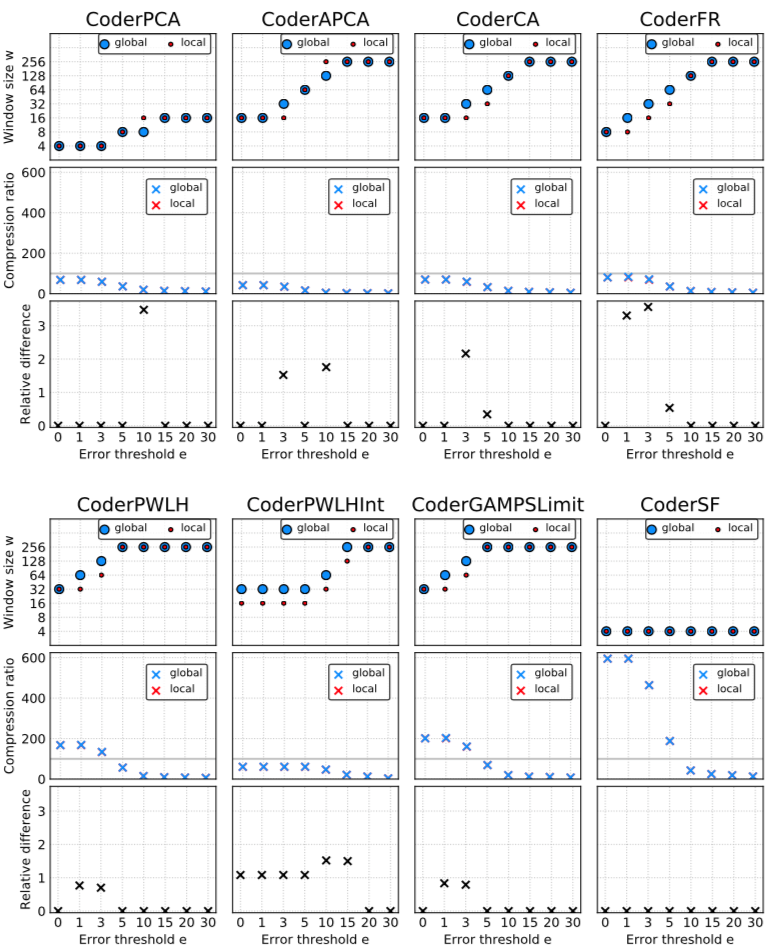
\includegraphics[clip,trim=0 0 0 0,height=22.5cm]{chapters/Experiments/images/3.3/1202.png}
\hspace{+5pt}
\caption{Global vs. local OWS, compression ratio and relative difference plots for every\\coding algorithm $a \in A$, for the ``VWC" data type of the ``vwc\_1202.dat.csv" file of the \datasetirkis \ dataset.}
\label{fig:window-compare-1202}
\end{figure}


\clearpage

\begin{figure}
\hspace{-70pt}
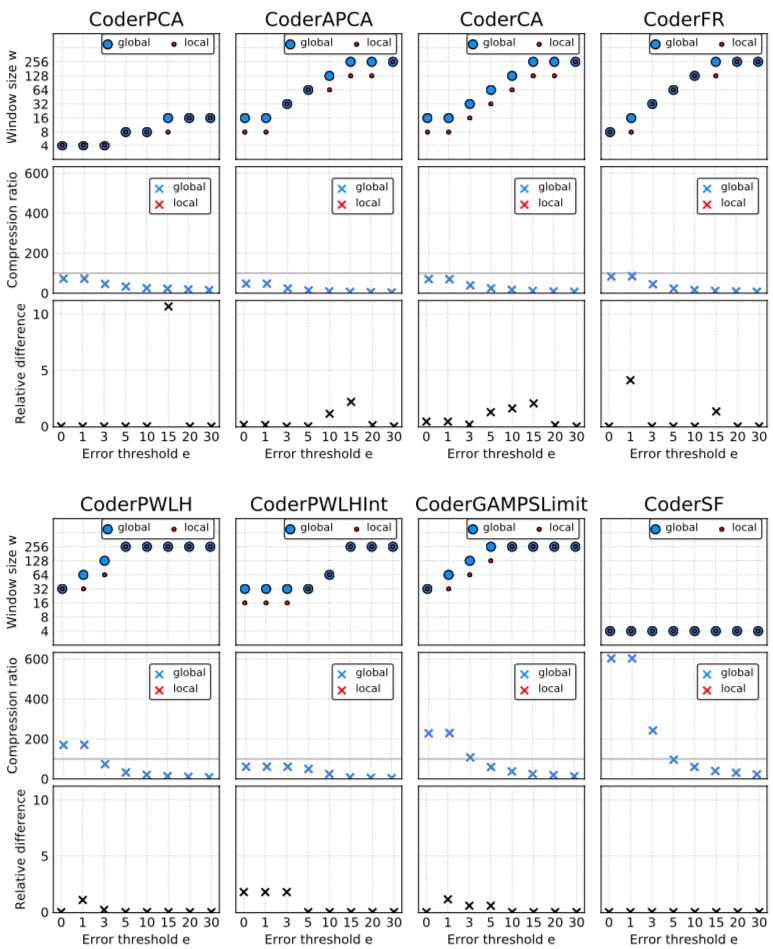
\includegraphics[clip,trim=0 0 0 0,height=22.5cm]{chapters/Experiments/images/3.3/1203.png}
\hspace{+5pt}
\caption{Global vs. local OWS, compression ratio and relative difference plots for every\\coding algorithm $a \in A$, for the ``VWC" data type of the ``vwc\_1203.dat.csv" file of the \datasetirkis \ dataset.}
\label{fig:window-compare-1203}
\end{figure}


\clearpage